\chapter{Principales interfaces du prototype}
\label{appendix:frontend-gallery}

Les captures de cette annexe sont produites par un sc\'enario Playwright d\'edi\'e,
adoss\'e au backend E2E et \`a une base temporaire. Le sc\'enario s'authentifie,
rejoue 40 observations d'attaque, attend leur persistance puis ouvre chaque vue.
Les compteurs constituent donc la preuve de cette ex\'ecution born\'ee, et non des
mesures de production. Les images sont captur\'ees \`a haute densit\'e apr\`es
chargement des polices, stabilisation des graphiques et remise \`a z\'ero du
d\'efilement.

\section{Supervision op\'erationnelle}

La vue de supervision synth\'etise l'\'etat du capteur passif, la fen\^etre
d'observation, les volumes persist\'es et la charge d'investigation. Elle s\'epare
les compteurs du capteur Suricata des pr\'edictions issues du mod\`ele. Le capteur
reste hors ligne dans cette capture car le sc\'enario rejoue des observations de
mod\`ele sans d\'emarrer le laboratoire de paquets.

\begin{figure}[htbp]
  \centering
  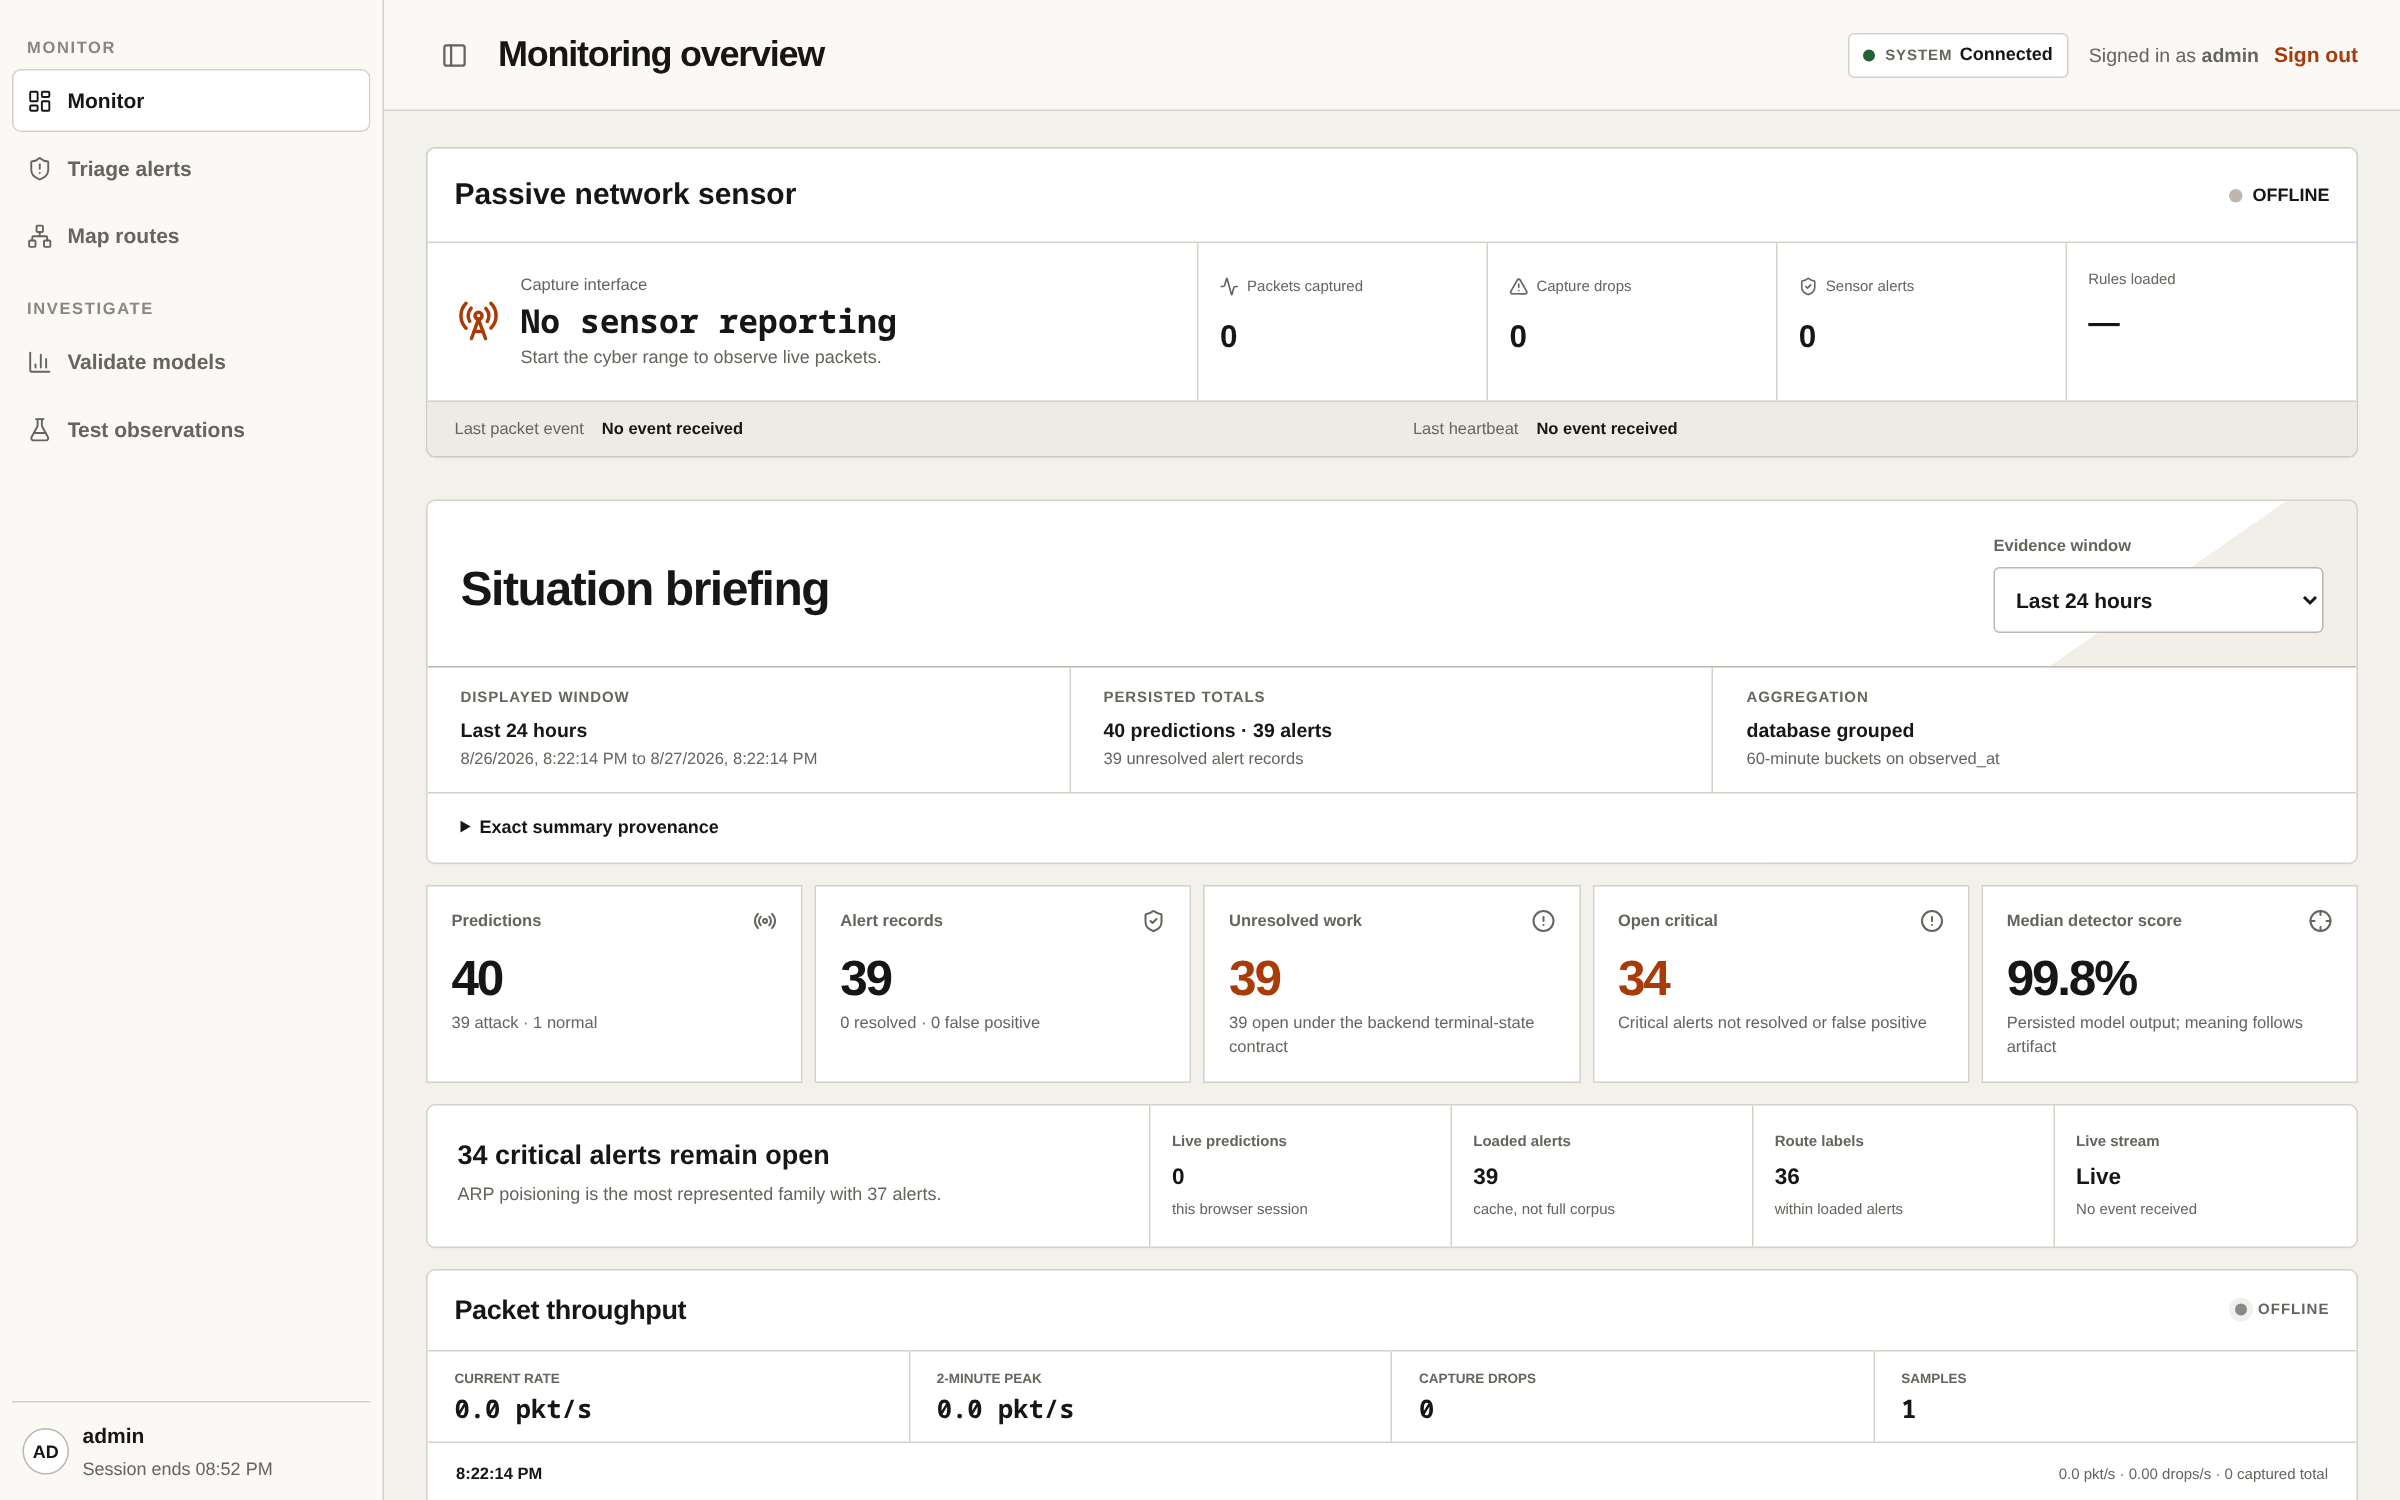
\includegraphics[width=\textwidth]{assets/screenshots/application-monitoring.png}
  \caption{Vue principale de supervision pendant un sc\'enario Playwright aliment\'e}
  \label{fig:frontend-monitoring}
\end{figure}

\clearpage
\section{Investigation des alertes}

L'espace d'investigation permet de filtrer les alertes selon le temps, la
d\'etection, la s\'ev\'erit\'e et le statut. La recherche et la pagination sont
effectu\'ees par le backend afin de conserver un comportement born\'e lorsque le
nombre d'enregistrements augmente.

\begin{figure}[htbp]
  \centering
  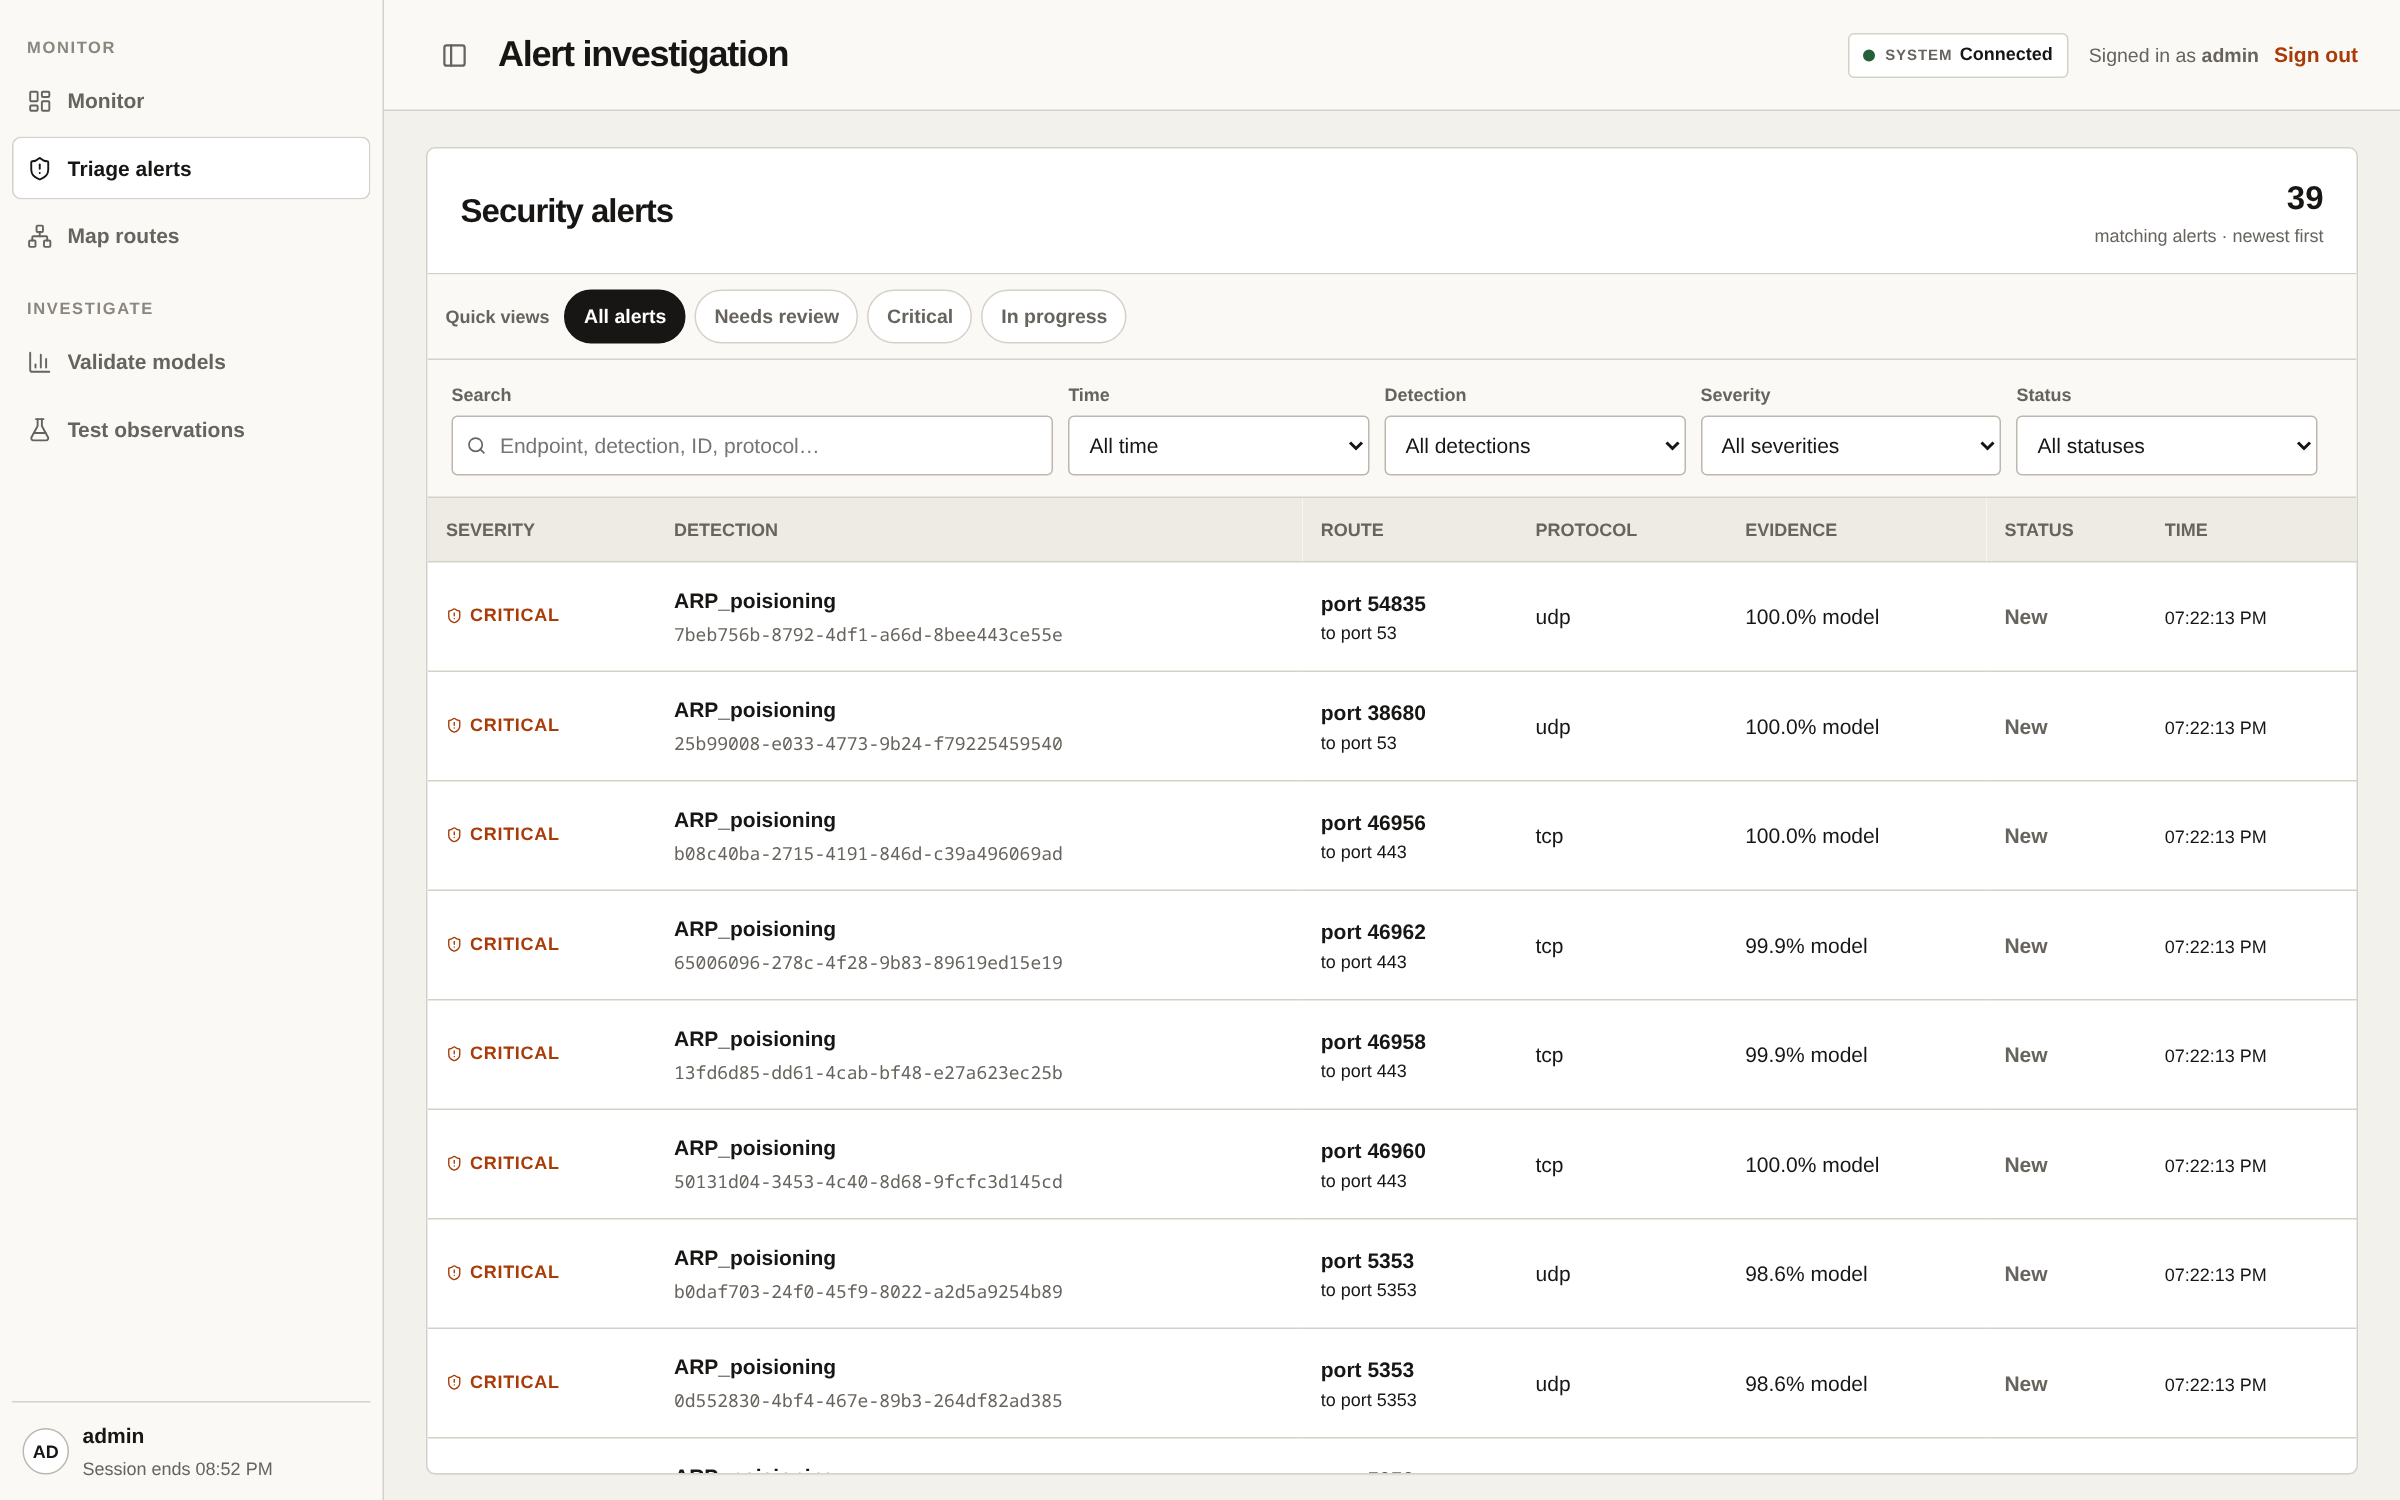
\includegraphics[width=\textwidth]{assets/screenshots/application-alert-investigation.png}
  \caption{Liste filtrable des alertes de s\'ecurit\'e dans l'interface d'investigation}
  \label{fig:frontend-alert-investigation}
\end{figure}

\clearpage
\section{Cartographie des communications}

La cartographie construit des relations \`a partir du cache d'alertes charg\'e et
en affiche explicitement le p\'erim\`etre. Les extr\'emit\'es identifi\'ees seulement
par un port restent signal\'ees comme observations limit\'ees; elles ne sont pas
pr\'esent\'ees comme des appareils confirm\'es.

\begin{figure}[htbp]
  \centering
  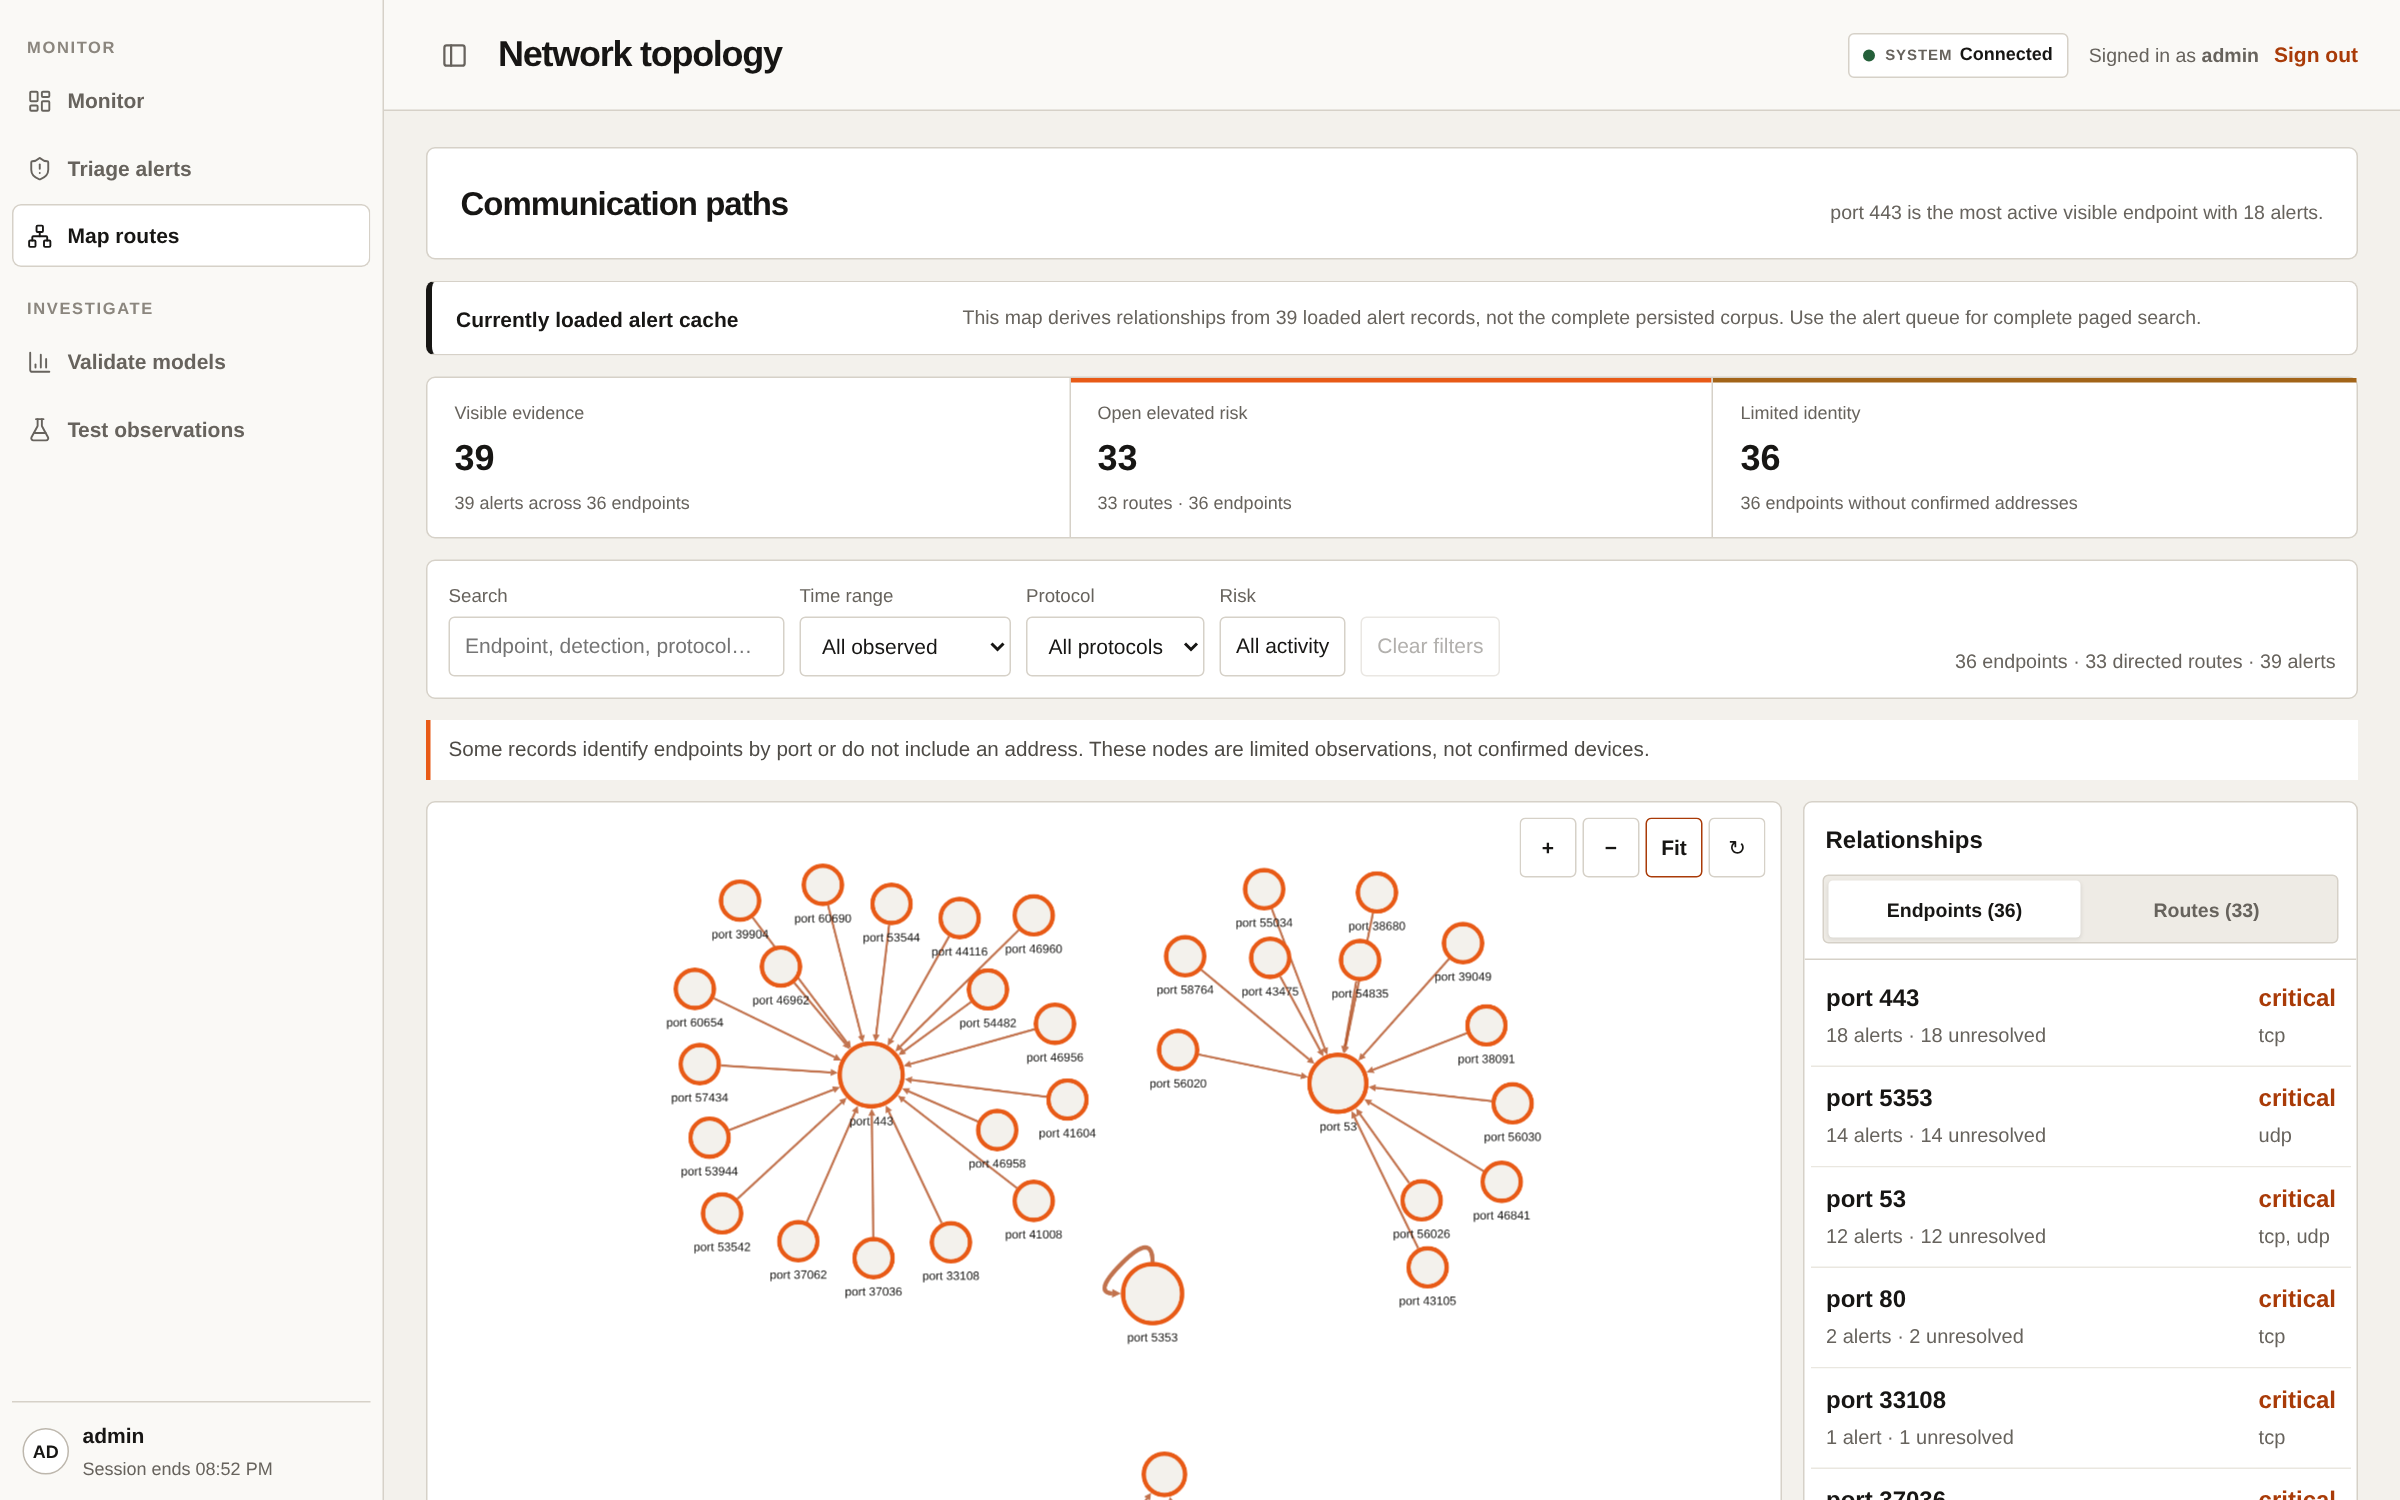
\includegraphics[width=\textwidth]{assets/screenshots/application-topology.png}
  \caption{Cartographie des routes d\'eriv\'ee des alertes charg\'ees pendant le sc\'enario E2E}
  \label{fig:frontend-topology}
\end{figure}

\clearpage
\section{Laboratoire d'observations}

Le laboratoire d'observations pr\'esente le contrat de donn\'ees attendu avant
toute soumission. La s\'election et l'inspection initiale du fichier restent
locales au navigateur; l'envoi vers le backend exige ensuite une session
authentifi\'ee.

\begin{figure}[htbp]
  \centering
  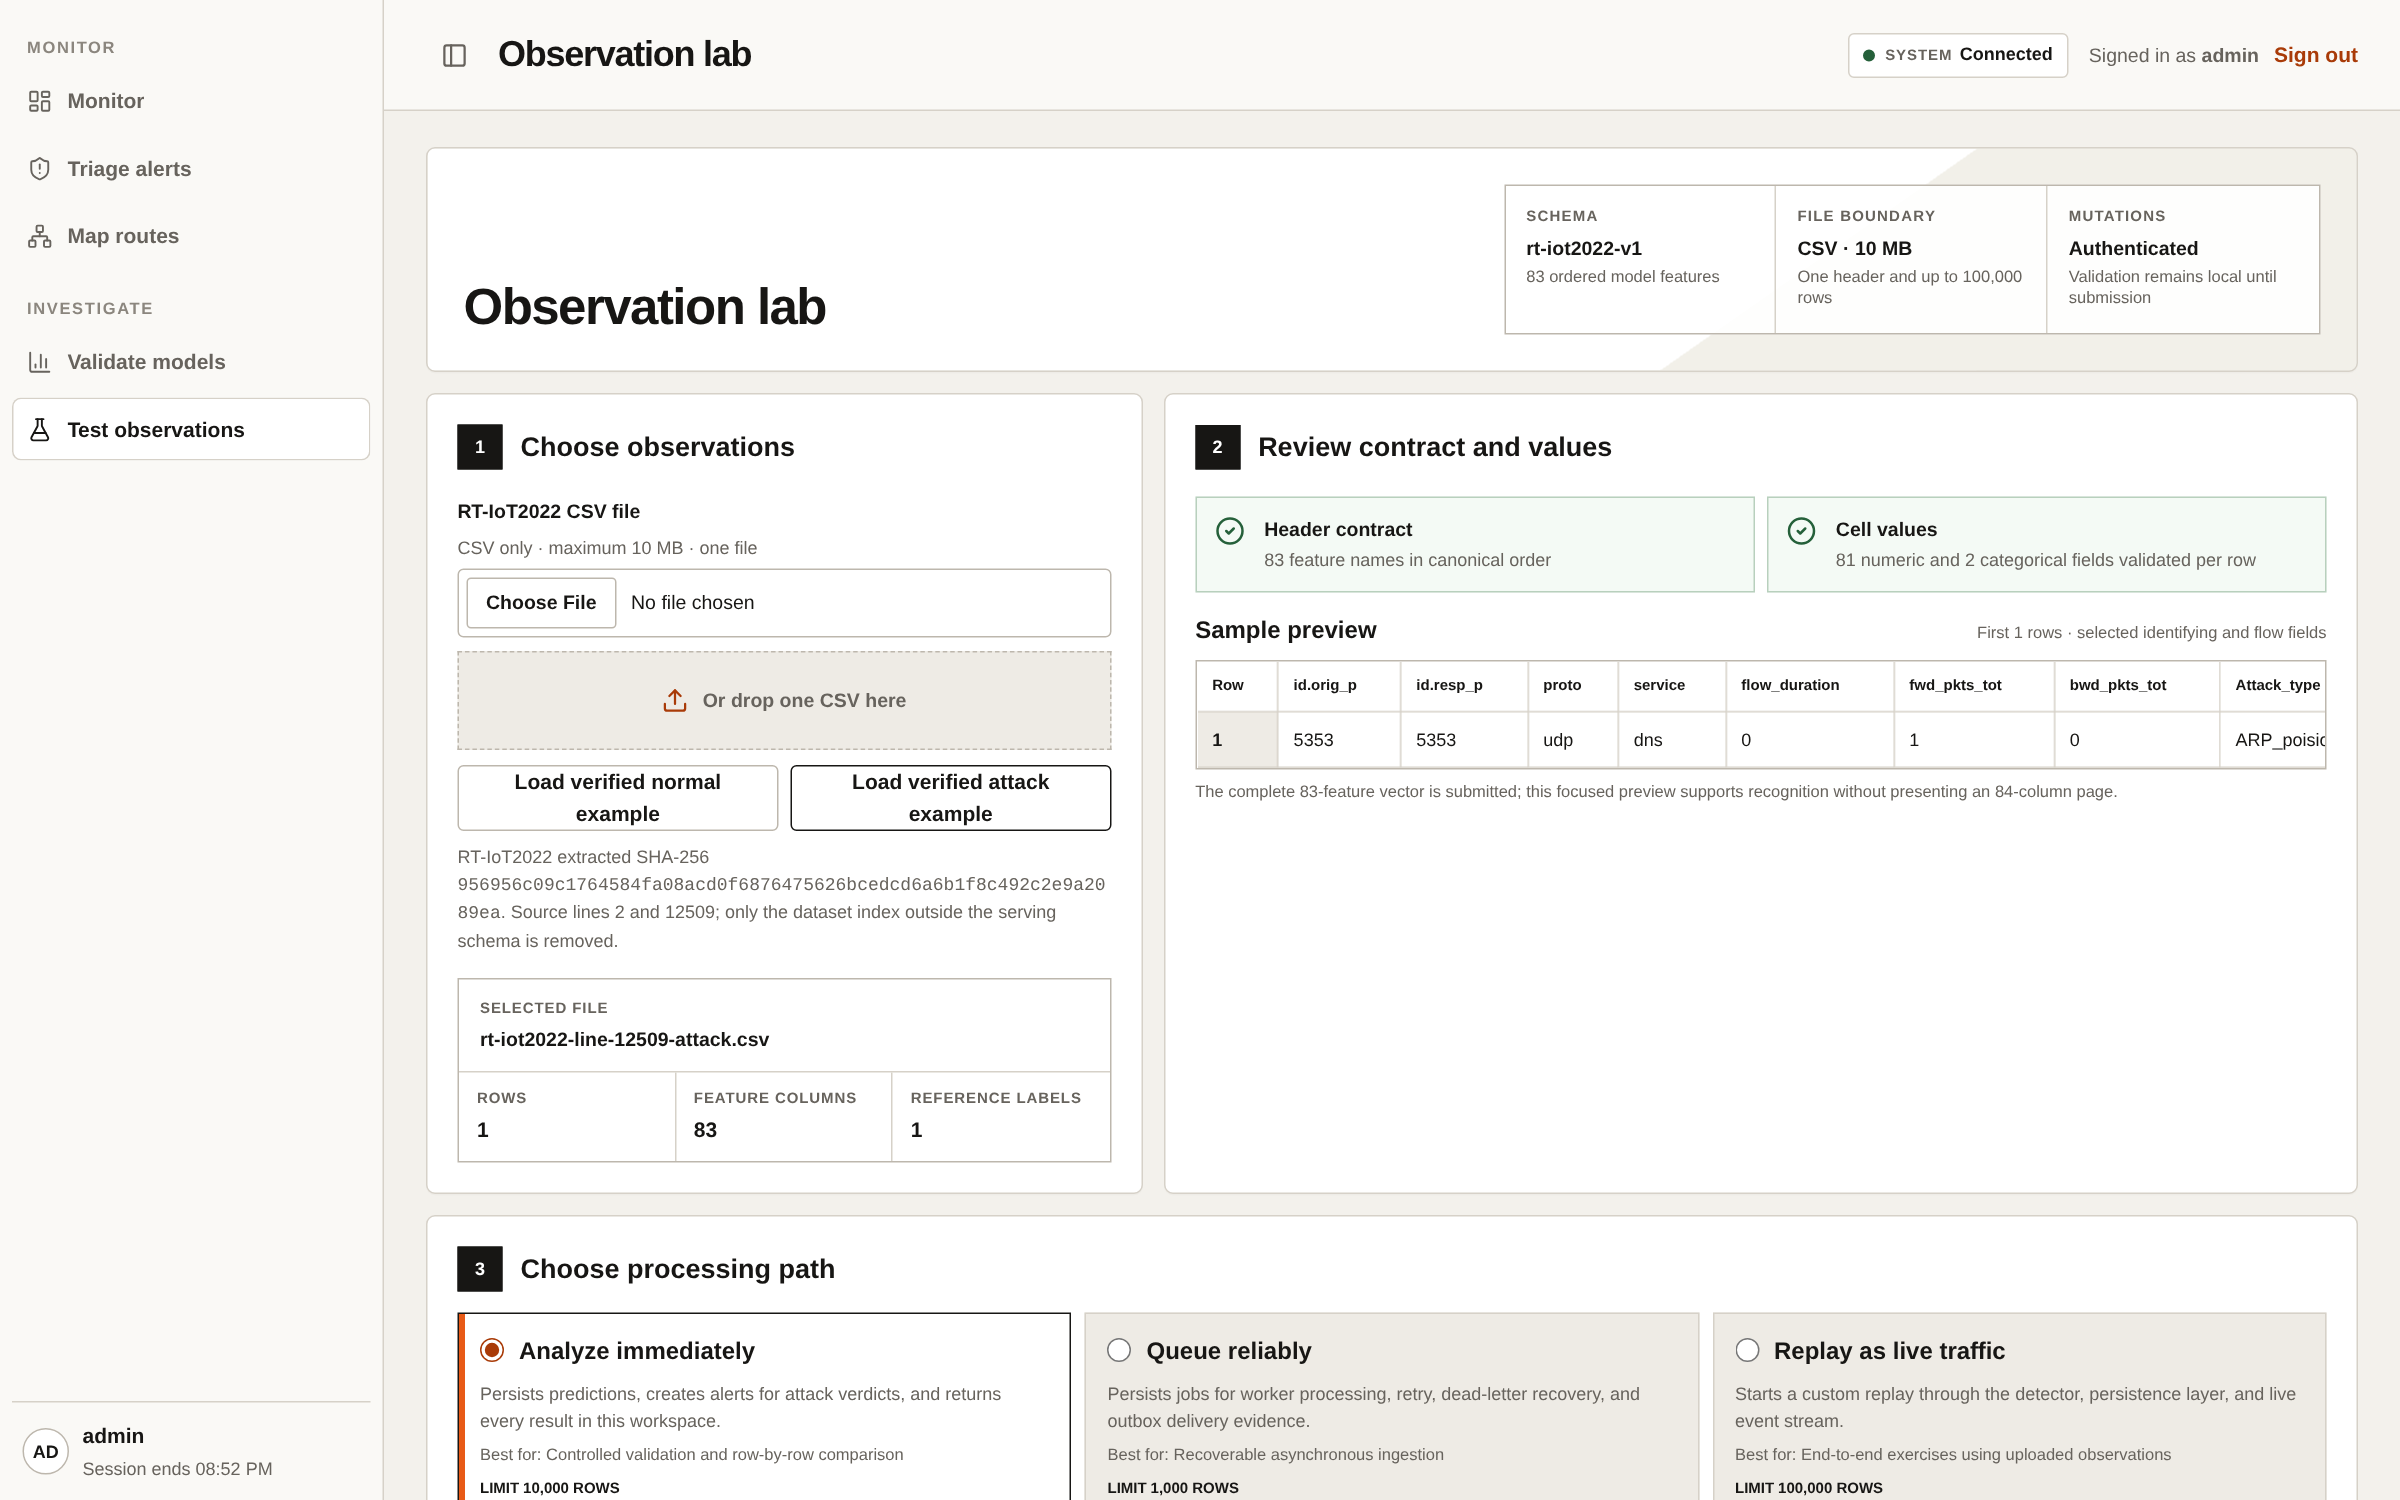
\includegraphics[width=\textwidth]{assets/screenshots/application-observation-lab.png}
  \caption{Contr\^ole local d'un exemple d'attaque conforme au sch\'ema RT-IoT2022}
  \label{fig:frontend-observation-lab}
\end{figure}

\clearpage
\section{Adaptation aux petits \'ecrans}

La navigation principale se replie derri\`ere un bouton d'ouverture sur petit
\'ecran. Les filtres et les alertes deviennent verticaux afin d'\'eviter tout
d\'efilement horizontal, tout en conservant les m\^emes libell\'es et \'etats que
sur la vue de bureau.

\begin{figure}[htbp]
  \centering
  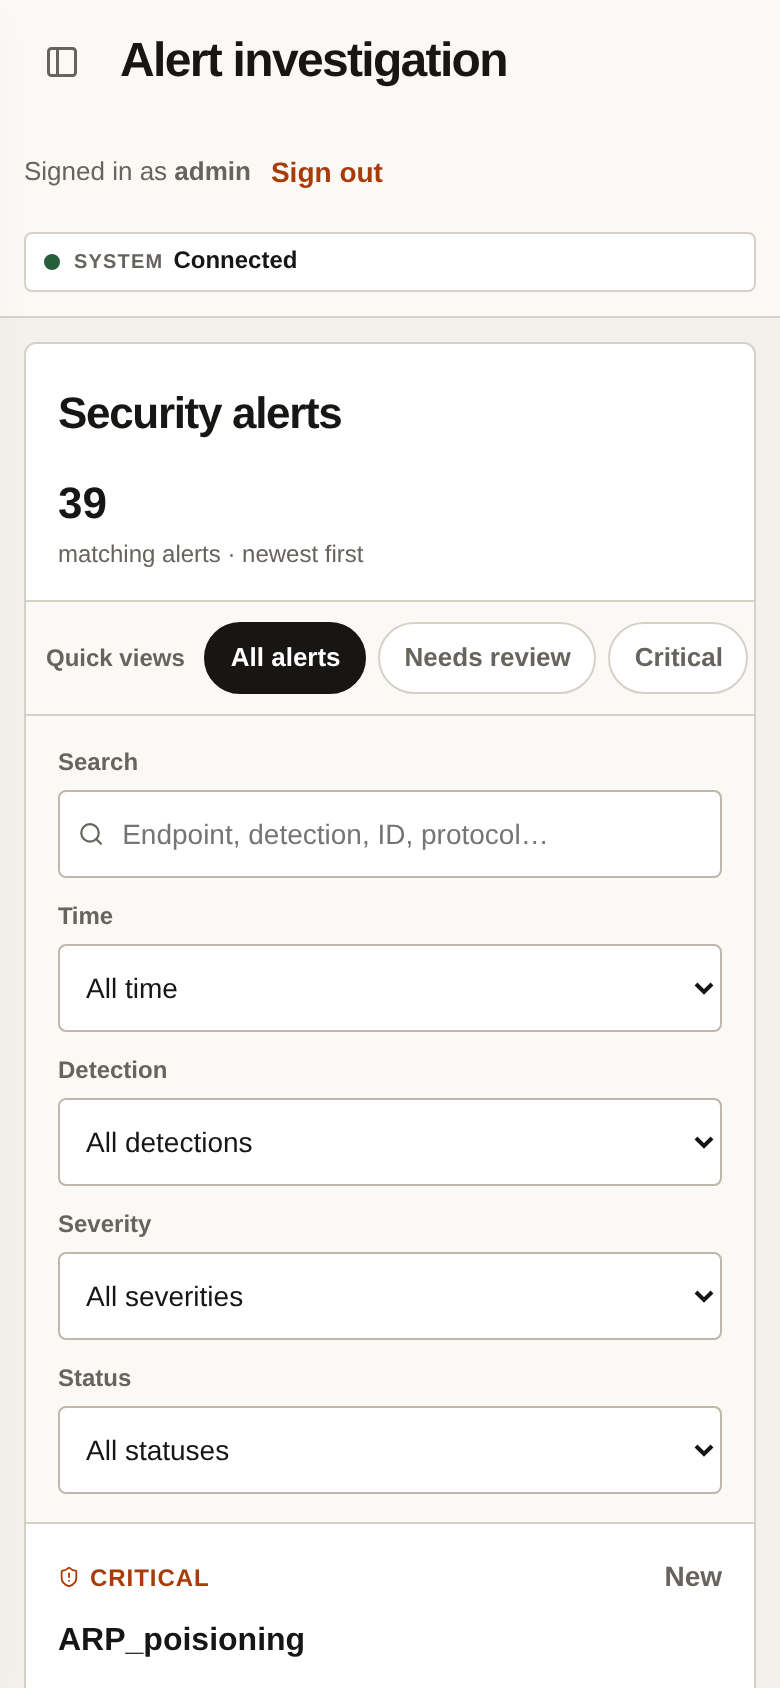
\includegraphics[height=0.68\textheight]{assets/screenshots/application-alerts-mobile.png}
  \caption{Espace d'investigation adapt\'e \`a une largeur mobile de 390 pixels}
  \label{fig:frontend-alerts-mobile}
\end{figure}
